% This file was created with tikzplotlib v0.10.1.
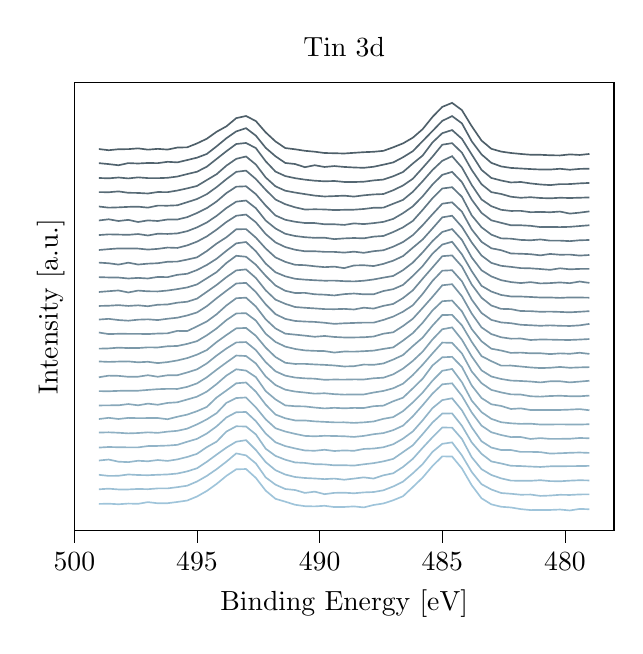
\begin{tikzpicture}

\definecolor{darkgray133164181}{RGB}{133,164,181}
\definecolor{darkgray136168186}{RGB}{136,168,186}
\definecolor{darkgray139172190}{RGB}{139,172,190}
\definecolor{darkgray143176195}{RGB}{143,176,195}
\definecolor{darkgray146180200}{RGB}{146,180,200}
\definecolor{darkgray176}{RGB}{176,176,176}
\definecolor{dimgray7895105}{RGB}{78,95,105}
\definecolor{dimgray8199110}{RGB}{81,99,110}
\definecolor{dimgray84103114}{RGB}{84,103,114}
\definecolor{dimgray88107118}{RGB}{88,107,118}
\definecolor{dimgray91111123}{RGB}{91,111,123}
\definecolor{lightslategray114139154}{RGB}{114,139,154}
\definecolor{lightslategray117143159}{RGB}{117,143,159}
\definecolor{lightslategray120147163}{RGB}{120,147,163}
\definecolor{lightslategray123152168}{RGB}{123,152,168}
\definecolor{lightslategray126156172}{RGB}{126,156,172}
\definecolor{lightslategray130160177}{RGB}{130,160,177}
\definecolor{lightsteelblue149184204}{RGB}{149,184,204}
\definecolor{lightsteelblue152188209}{RGB}{152,188,209}
\definecolor{lightsteelblue156192213}{RGB}{156,192,213}
\definecolor{lightsteelblue159196218}{RGB}{159,196,218}
\definecolor{slategray101123137}{RGB}{101,123,137}
\definecolor{slategray104127141}{RGB}{104,127,141}
\definecolor{slategray107131146}{RGB}{107,131,146}
\definecolor{slategray110135150}{RGB}{110,135,150}
\definecolor{slategray94115128}{RGB}{94,115,128}
\definecolor{slategray97119132}{RGB}{97,119,132}

\begin{axis}[
scaled y ticks=manual:{}{\pgfmathparse{#1}},
tick align=outside,
title={Tin 3d},
x dir=reverse,
x grid style={darkgray176},
xlabel={Binding Energy [eV]},
xmin=478, xmax=500,
xtick pos=left,
xtick style={color=black},
y grid style={darkgray176},
ylabel={Intensity [a.u.]},
ymajorticks=false,
ymin=-96949.3, ymax=61853.3,
ytick style={color=black},
yticklabels={}
]
\addplot [semithick, dimgray7895105]
table {%
499 38284
498.6 37865
498.2 38220
497.8 38245
497.4 38522
497 38066
496.6 38347
496.2 38091
495.8 38810
495.4 38890
495 40275
494.6 41923
494.2 44402
493.8 46323
493.4 49229
493 49987
492.6 48193
492.2 44195
491.8 40973
491.4 38630
491 38200
490.6 37661
490.2 37338
489.8 36875
489.4 36802
489 36700
488.6 36945
488.2 37171
487.8 37313
487.4 37641
487 38904
486.6 40289
486.2 42305
485.8 45328
485.4 49642
485 53214
484.6 54635
484.2 52067
483.8 46373
483.4 41286
483 38366
482.6 37384
482.2 36879
481.8 36545
481.4 36259
481 36249
480.6 36082
480.2 36018
479.8 36387
479.4 36183
479 36544
};
\addplot [semithick, dimgray8199110]
table {%
499 33288
498.6 32949
498.2 32540
497.8 33301
497.4 33163
497 33351
496.6 33287
496.2 33762
495.8 33560
495.4 34381
495 35223
494.6 36540
494.2 39239
493.8 42121
493.4 44536
493 45670
492.6 43028
492.2 38720
491.8 35721
491.4 33354
491 32972
490.6 31851
490.2 32550
489.8 31930
489.4 32256
489 31944
488.6 31753
488.2 31634
487.8 32009
487.4 32748
487 33542
486.6 35375
486.2 37533
485.8 41100
485.4 44659
485 48255
484.6 49957
484.2 47381
483.8 41040
483.4 36384
483 33386
482.6 32119
482.2 31597
481.8 31393
481.4 31194
481 31030
480.6 31018
480.2 31293
479.8 30948
479.4 31247
479 31327
};
\addplot [semithick, dimgray84103114]
table {%
499 28033
498.6 27908
498.2 28203
497.8 27878
497.4 28253
497 27991
496.6 27967
496.2 28096
495.8 28545
495.4 29415
495 30241
494.6 32029
494.2 34777
493.8 37518
493.4 40069
493 40433
492.6 38615
492.2 33957
491.8 30294
491.4 28707
491 27962
490.6 27440
490.2 27067
489.8 26859
489.4 26965
489 26632
488.6 26604
488.2 26710
487.8 27172
487.4 27469
487 28643
486.6 30154
486.2 33155
485.8 35980
485.4 40613
485 43901
484.6 45009
484.2 41899
483.8 36366
483.4 30897
483 28044
482.6 27138
482.2 26447
481.8 26618
481.4 26103
481 25734
480.6 25509
480.2 25859
479.8 25874
479.4 26127
479 26275
};
\addplot [semithick, dimgray88107118]
table {%
499 23032
498.6 22983
498.2 23276
497.8 22791
497.4 22733
497 22536
496.6 23058
496.2 23010
495.8 23587
495.4 24345
495 25201
494.6 27303
494.2 29369
493.8 32405
493.4 34812
493 35648
492.6 32806
492.2 28219
491.8 25083
491.4 23518
491 22870
490.6 22317
490.2 21792
489.8 21482
489.4 21613
489 21767
488.6 21446
488.2 21894
487.8 22203
487.4 22351
487 23696
486.6 25379
486.2 27760
485.8 31613
485.4 35557
485 39815
484.6 40370
484.2 37006
483.8 30883
483.4 25821
483 23020
482.6 22366
482.2 21384
481.8 21020
481.4 21222
481 20941
480.6 20823
480.2 21032
479.8 20935
479.4 21039
479 21143
};
\addplot [semithick, dimgray91111123]
table {%
499 17929
498.6 17521
498.2 17625
497.8 17801
497.4 17869
497 17530
496.6 18243
496.2 18217
495.8 18365
495.4 19457
495 20568
494.6 22299
494.2 24788
493.8 27623
493.4 30208
493 30639
492.6 27661
492.2 23857
491.8 20405
491.4 18737
491 17641
490.6 16867
490.2 16943
489.8 16884
489.4 16667
489 16757
488.6 16805
488.2 17050
487.8 17483
487.4 17523
487 18905
486.6 20282
486.2 23147
485.8 26887
485.4 30847
485 34113
484.6 35748
484.2 31745
483.8 25557
483.4 20420
483 18043
482.6 16762
482.2 16361
481.8 16383
481.4 15914
481 16014
480.6 15898
480.2 16139
479.8 15415
479.4 15758
479 16202
};
\addplot [semithick, slategray94115128]
table {%
499 12983
498.6 13404
498.2 12792
497.8 13199
497.4 12438
497 13009
496.6 12797
496.2 13325
495.8 13323
495.4 14153
495 15623
494.6 17346
494.2 19708
493.8 22682
493.4 24950
493 25090
492.6 22306
492.2 18267
491.8 14761
491.4 13231
491 12524
490.6 12088
490.2 12062
489.8 11641
489.4 11642
489 11404
488.6 11948
488.2 11702
487.8 12042
487.4 12486
487 13542
486.6 15576
486.2 17990
485.8 21531
485.4 25702
485 29145
484.6 30195
484.2 26577
483.8 20364
483.4 15670
483 13042
482.6 12151
482.2 11278
481.8 11284
481.4 11088
481 10640
480.6 10682
480.2 10632
479.8 10726
479.4 11013
479 11292
};
\addplot [semithick, slategray97119132]
table {%
499 7816
498.6 8064
498.2 7989
497.8 7897
497.4 8179
497 7664
496.6 8287
496.2 8215
495.8 8401
495.4 9190
495 10531
494.6 12268
494.2 14610
493.8 17392
493.4 19645
493 20045
492.6 17336
492.2 12969
491.8 10149
491.4 8266
491 7484
490.6 7063
490.2 6831
489.8 6872
489.4 6374
489 6635
488.6 6770
488.2 6655
487.8 7255
487.4 7501
487 8891
486.6 10548
486.2 12830
485.8 16726
485.4 20842
485 24307
484.6 24759
484.2 21381
483.8 14794
483.4 10579
483 7959
482.6 6644
482.2 6529
481.8 6100
481.4 5966
481 6259
480.6 5833
480.2 5839
479.8 5664
479.4 5970
479 6067
};
\addplot [semithick, slategray101123137]
table {%
499 2520
498.6 2825
498.2 3078
497.8 3078
497.4 3025
497 2677
496.6 2921
496.2 3386
495.8 3258
495.4 4152
495 5478
494.6 7334
494.2 9736
493.8 12452
493.4 14658
493 15077
492.6 12335
492.2 8189
491.8 5220
491.4 3563
491 2619
490.6 2073
490.2 2085
489.8 1873
489.4 1846
489 1604
488.6 1934
488.2 1526
487.8 2101
487.4 2438
487 3703
486.6 5347
486.2 7789
485.8 11304
485.4 15177
485 18917
484.6 19414
484.2 16107
483.8 9813
483.4 5431
483 3130
482.6 2462
482.2 1293
481.8 1195
481.4 1041
481 623
480.6 1129
480.2 843
479.8 899
479.4 545
479 753
};
\addplot [semithick, slategray104127141]
table {%
499 -1944
498.6 -2168
498.2 -2643
497.8 -1965
497.4 -2621
497 -2314
496.6 -2159
496.2 -1645
495.8 -1578
495.4 -871
495 -89
494.6 2142
494.2 4799
493.8 7027
493.4 9862
493 9931
492.6 6909
492.2 3065
491.8 -105
491.4 -1676
491 -2719
490.6 -2847
490.2 -3238
489.8 -3549
489.4 -3365
489 -3899
488.6 -2953
488.2 -2863
487.8 -3168
487.4 -2391
487 -1246
486.6 369
486.2 3342
485.8 6250
485.4 10142
485 14092
484.6 14658
484.2 10716
483.8 5192
483.4 569
483 -2035
482.6 -3079
482.2 -3454
481.8 -3885
481.4 -3967
481 -4210
480.6 -4501
480.2 -3957
479.8 -4315
479.4 -4175
479 -4168
};
\addplot [semithick, slategray107131146]
table {%
499 -7091
498.6 -7196
498.2 -7234
497.8 -7568
497.4 -7351
497 -7570
496.6 -7018
496.2 -7094
495.8 -6269
495.4 -5897
495 -4569
494.6 -2777
494.2 -578
493.8 2249
493.4 4881
493 5351
492.6 2084
492.2 -2294
491.8 -5368
491.4 -6796
491 -7674
490.6 -7977
490.2 -8187
489.8 -8349
489.4 -8319
489 -8511
488.6 -8601
488.2 -8362
487.8 -7912
487.4 -7265
487 -6658
486.6 -4614
486.2 -1931
485.8 1681
485.4 5668
485 8915
484.6 9932
484.2 6116
483.8 -113
483.4 -4655
483 -6828
482.6 -8163
482.2 -8831
481.8 -9189
481.4 -8853
481 -9316
480.6 -9192
480.2 -8963
479.8 -9232
479.4 -8639
479 -9129
};
\addplot [semithick, slategray110135150]
table {%
499 -12353
498.6 -12067
498.2 -11804
497.8 -12518
497.4 -11848
497 -12105
496.6 -12150
496.2 -11838
495.8 -11327
495.4 -10736
495 -9671
494.6 -7497
494.2 -5308
493.8 -2073
493.4 482
493 131
492.6 -2692
492.2 -6619
491.8 -10042
491.4 -11934
491 -12711
490.6 -12660
490.2 -13154
489.8 -13298
489.4 -13571
489 -13104
488.6 -12892
488.2 -13164
487.8 -13153
487.4 -12008
487 -11349
486.6 -9840
486.2 -6653
485.8 -3157
485.4 1220
485 4450
484.6 5441
484.2 990
483.8 -4962
483.4 -10160
483 -12187
482.6 -13401
482.2 -13934
481.8 -13950
481.4 -14116
481 -14298
480.6 -14293
480.2 -14436
479.8 -14271
479.4 -14302
479 -14367
};
\addplot [semithick, lightslategray114139154]
table {%
499 -17294
498.6 -17213
498.2 -17004
497.8 -17290
497.4 -17070
497 -17397
496.6 -16870
496.2 -16768
495.8 -16136
495.4 -15805
495 -14705
494.6 -12287
494.2 -9850
493.8 -7101
493.4 -4698
493 -4346
492.6 -7381
492.2 -11750
491.8 -15053
491.4 -16541
491 -17668
490.6 -17939
490.2 -18156
489.8 -18402
489.4 -18443
489 -18334
488.6 -18548
488.2 -17904
487.8 -18227
487.4 -17260
487 -16577
486.6 -14499
486.2 -11755
485.8 -7659
485.4 -3663
485 333
484.6 608
484.2 -3319
483.8 -9702
483.4 -14381
483 -17141
482.6 -18327
482.2 -18420
481.8 -19098
481.4 -19127
481 -19358
480.6 -19289
480.2 -19407
479.8 -19549
479.4 -19349
479 -19140
};
\addplot [semithick, lightslategray117143159]
table {%
499 -22108
498.6 -21858
498.2 -22286
497.8 -22515
497.4 -22156
497 -22031
496.6 -22297
496.2 -21825
495.8 -21455
495.4 -20663
495 -19595
494.6 -17388
494.2 -14568
493.8 -11904
493.4 -9336
493 -9126
492.6 -12378
492.2 -16714
491.8 -20196
491.4 -21874
491 -22608
490.6 -22816
490.2 -22947
489.8 -23245
489.4 -23639
489 -23435
488.6 -23312
488.2 -23191
487.8 -23209
487.4 -22242
487 -21055
486.6 -19323
486.2 -17040
485.8 -13030
485.4 -8433
485 -4804
484.6 -4638
484.2 -8543
483.8 -15043
483.4 -19787
483 -22226
482.6 -23128
482.2 -23404
481.8 -23962
481.4 -24122
481 -24316
480.6 -24169
480.2 -24324
479.8 -24381
479.4 -24163
479 -23647
};
\addplot [semithick, lightslategray120147163]
table {%
499 -26699
498.6 -27259
498.2 -27153
497.8 -27171
497.4 -27173
497 -27248
496.6 -27063
496.2 -26991
495.8 -26126
495.4 -26195
495 -24544
494.6 -22793
494.2 -20240
493.8 -17116
493.4 -14553
493 -14365
492.6 -17480
492.2 -22011
491.8 -25249
491.4 -27109
491 -27451
490.6 -27810
490.2 -28208
489.8 -27922
489.4 -28275
489 -28453
488.6 -28447
488.2 -28379
487.8 -28123
487.4 -27114
487 -26622
486.6 -24395
486.2 -21829
485.8 -17994
485.4 -14071
485 -9977
484.6 -9587
484.2 -13855
483.8 -19988
483.4 -24885
483 -27258
482.6 -28382
482.2 -28885
481.8 -28835
481.4 -29353
481 -29175
480.6 -29216
480.2 -29313
479.8 -29339
479.4 -29193
479 -29011
};
\addplot [semithick, lightslategray123152168]
table {%
499 -32421
498.6 -32329
498.2 -32063
497.8 -32216
497.4 -32198
497 -31956
496.6 -31999
496.2 -31574
495.8 -31469
495.4 -30731
495 -29762
494.6 -27690
494.2 -25257
493.8 -22311
493.4 -19948
493 -19864
492.6 -22465
492.2 -27130
491.8 -30041
491.4 -31694
491 -32527
490.6 -33030
490.2 -33202
489.8 -33279
489.4 -33801
489 -33433
488.6 -33482
488.2 -33313
487.8 -33111
487.4 -32512
487 -31966
486.6 -29560
486.2 -26916
485.8 -23238
485.4 -18912
485 -15610
484.6 -15377
484.2 -19195
483.8 -25481
483.4 -29801
483 -32437
482.6 -33076
482.2 -33930
481.8 -33816
481.4 -34070
481 -34045
480.6 -34344
480.2 -34087
479.8 -34236
479.4 -33868
479 -34283
};
\addplot [semithick, lightslategray126156172]
table {%
499 -36951
498.6 -37112
498.2 -36995
497.8 -36936
497.4 -37254
497 -37066
496.6 -37535
496.2 -37176
495.8 -36597
495.4 -35769
495 -34542
494.6 -32922
494.2 -30089
493.8 -27593
493.4 -25223
493 -25080
492.6 -27864
492.2 -32046
491.8 -35380
491.4 -37421
491 -37828
490.6 -37810
490.2 -38009
489.8 -38161
489.4 -38377
489 -38728
488.6 -38626
488.2 -38050
487.8 -38148
487.4 -37659
487 -36282
486.6 -34672
486.2 -31498
485.8 -28505
485.4 -24264
485 -20505
484.6 -20449
484.2 -24160
483.8 -30002
483.4 -35060
483 -36847
482.6 -38427
482.2 -38410
481.8 -38744
481.4 -39072
481 -39294
480.6 -39190
480.2 -38897
479.8 -39188
479.4 -39052
479 -38968
};
\addplot [semithick, lightslategray130160177]
table {%
499 -42555
498.6 -41979
498.2 -42051
497.8 -42386
497.4 -42351
497 -41826
496.6 -42372
496.2 -41845
495.8 -41827
495.4 -40852
495 -39750
494.6 -37654
494.2 -34867
493.8 -32360
493.4 -30216
493 -30085
492.6 -32920
492.2 -37191
491.8 -40431
491.4 -41977
491 -42654
490.6 -42934
490.2 -43059
489.8 -43445
489.4 -43357
489 -43390
488.6 -43305
488.2 -43337
487.8 -42910
487.4 -42705
487 -41513
486.6 -39491
486.2 -36752
485.8 -33478
485.4 -29182
485 -25548
484.6 -24892
484.2 -29247
483.8 -35176
483.4 -40102
483 -42280
482.6 -43157
482.2 -43722
481.8 -43867
481.4 -44061
481 -44374
480.6 -43982
480.2 -43967
479.8 -44365
479.4 -44085
479 -43790
};
\addplot [semithick, darkgray133164181]
table {%
499 -47463
498.6 -47503
498.2 -47369
497.8 -47300
497.4 -47315
497 -47030
496.6 -46770
496.2 -46656
495.8 -46684
495.4 -45954
495 -44724
494.6 -42569
494.2 -39869
493.8 -37318
493.4 -34855
493 -35030
492.6 -37653
492.2 -42258
491.8 -45296
491.4 -46947
491 -47610
490.6 -47966
490.2 -48358
489.8 -48217
489.4 -48529
489 -48698
488.6 -48634
488.2 -48637
487.8 -47955
487.4 -47391
487 -46457
486.6 -44826
486.2 -41757
485.8 -38105
485.4 -34108
485 -30265
484.6 -30361
484.2 -34103
483.8 -40500
483.4 -44640
483 -47026
482.6 -47911
482.2 -48607
481.8 -48673
481.4 -49281
481 -49413
480.6 -49188
480.2 -49098
479.8 -49257
479.4 -49284
479 -49044
};
\addplot [semithick, darkgray136168186]
table {%
499 -52538
498.6 -52495
498.2 -52482
497.8 -52041
497.4 -52487
497 -51888
496.6 -52291
496.2 -51647
495.8 -51413
495.4 -50437
495 -49435
494.6 -47638
494.2 -44958
493.8 -41955
493.4 -39724
493 -40188
492.6 -42495
492.2 -47455
491.8 -50386
491.4 -52521
491 -52800
490.6 -52883
490.2 -53276
489.8 -53583
489.4 -53372
489 -53550
488.6 -53400
488.2 -53445
487.8 -52797
487.4 -52603
487 -51045
486.6 -49784
486.2 -46477
485.8 -43064
485.4 -38380
485 -35483
484.6 -35317
484.2 -38880
483.8 -45463
483.4 -49901
483 -52123
482.6 -52711
482.2 -53788
481.8 -53572
481.4 -54150
481 -54142
480.6 -54165
480.2 -54133
479.8 -54010
479.4 -53832
479 -54240
};
\addplot [semithick, darkgray139172190]
table {%
499 -57348
498.6 -56915
498.2 -57332
497.8 -56947
497.4 -57036
497 -57001
496.6 -56987
496.2 -57413
495.8 -56535
495.4 -55781
495 -54570
494.6 -53066
494.2 -49725
493.8 -47235
493.4 -44691
493 -44406
492.6 -47648
492.2 -52219
491.8 -55750
491.4 -57078
491 -57839
490.6 -57851
490.2 -58171
489.8 -58351
489.4 -58517
489 -58513
488.6 -58713
488.2 -58524
487.8 -58211
487.4 -57272
487 -56659
486.6 -54550
486.2 -51456
485.8 -47972
485.4 -43777
485 -40255
484.6 -39617
484.2 -44299
483.8 -50817
483.4 -54888
483 -57276
482.6 -58483
482.2 -58852
481.8 -59057
481.4 -59005
481 -59286
480.6 -59265
480.2 -59237
479.8 -59270
479.4 -59297
479 -59188
};
\addplot [semithick, darkgray143176195]
table {%
499 -62130
498.6 -62052
498.2 -62206
497.8 -62424
497.4 -62302
497 -62055
496.6 -62247
496.2 -61817
495.8 -61521
495.4 -60751
495 -59247
494.6 -57469
494.2 -55256
493.8 -51612
493.4 -49909
493 -49710
492.6 -53208
492.2 -57444
491.8 -60592
491.4 -61770
491 -62595
490.6 -63320
490.2 -63459
489.8 -63289
489.4 -63354
489 -63447
488.6 -63681
488.2 -63323
487.8 -62722
487.4 -62321
487 -61283
486.6 -59680
486.2 -56382
485.8 -52450
485.4 -48347
485 -45054
484.6 -44698
484.2 -49140
483.8 -55025
483.4 -59689
483 -62024
482.6 -63006
482.2 -63741
481.8 -63720
481.4 -64407
481 -64098
480.6 -64384
480.2 -64363
479.8 -64330
479.4 -64055
479 -64168
};
\addplot [semithick, darkgray146180200]
table {%
499 -67456
498.6 -67248
498.2 -67341
497.8 -67377
497.4 -67384
497 -66924
496.6 -66868
496.2 -66744
495.8 -66490
495.4 -65390
495 -64373
494.6 -62476
494.2 -59949
493.8 -56775
493.4 -54939
493 -54857
492.6 -58091
492.2 -62482
491.8 -65583
491.4 -66929
491 -67763
490.6 -68481
490.2 -68585
489.8 -68233
489.4 -68671
489 -68460
488.6 -68601
488.2 -67941
487.8 -67795
487.4 -67341
487 -66276
486.6 -64291
486.2 -61731
485.8 -57801
485.4 -53493
485 -50644
484.6 -49996
484.2 -54238
483.8 -60278
483.4 -65222
483 -67452
482.6 -68319
482.2 -68326
481.8 -68989
481.4 -68973
481 -69069
480.6 -69582
480.2 -69463
479.8 -69303
479.4 -69206
479 -69348
};
\addplot [semithick, lightsteelblue149184204]
table {%
499 -72036
498.6 -71690
498.2 -72456
497.8 -72609
497.4 -72123
497 -72306
496.6 -71865
496.2 -72182
495.8 -71644
495.4 -70786
495 -69669
494.6 -67307
494.2 -65349
493.8 -61774
493.4 -59916
493 -59990
492.6 -62781
492.2 -67852
491.8 -70394
491.4 -71753
491 -72723
490.6 -72897
490.2 -73329
489.8 -73406
489.4 -73738
489 -73703
488.6 -73833
488.2 -73374
487.8 -72968
487.4 -72340
487 -71465
486.6 -69060
486.2 -66633
485.8 -62696
485.4 -58590
485 -55409
484.6 -55345
484.2 -59727
483.8 -65636
483.4 -69663
483 -72356
482.6 -73087
482.2 -73903
481.8 -74000
481.4 -74177
481 -74320
480.6 -74097
480.2 -74081
479.8 -74023
479.4 -74003
479 -73932
};
\addplot [semithick, lightsteelblue152188209]
table {%
499 -77094
498.6 -77490
498.2 -77447
497.8 -76981
497.4 -77175
497 -77245
496.6 -77093
496.2 -76968
495.8 -76651
495.4 -75886
495 -74785
494.6 -72495
494.2 -69946
493.8 -67467
493.4 -65373
493 -64827
492.6 -68293
492.2 -72589
491.8 -75464
491.4 -77006
491 -77882
490.6 -78233
490.2 -78400
489.8 -78628
489.4 -78442
489 -78838
488.6 -78441
488.2 -78004
487.8 -78436
487.4 -77282
487 -76551
486.6 -74308
486.2 -71440
485.8 -67544
485.4 -63800
485 -60351
484.6 -60396
484.2 -64385
483.8 -70865
483.4 -75101
483 -77160
482.6 -78363
482.2 -79157
481.8 -79216
481.4 -79221
481 -79011
480.6 -79331
480.2 -79393
479.8 -79169
479.4 -79025
479 -79104
};
\addplot [semithick, lightsteelblue156192213]
table {%
499 -82232
498.6 -82012
498.2 -82284
497.8 -82282
497.4 -82110
497 -82195
496.6 -81921
496.2 -81914
495.8 -81473
495.4 -80961
495 -79472
494.6 -77496
494.2 -75105
493.8 -72434
493.4 -69517
493 -70215
492.6 -73069
492.2 -78009
491.8 -80583
491.4 -82132
491 -82485
490.6 -83513
490.2 -83061
489.8 -83958
489.4 -83500
489 -83433
488.6 -83644
488.2 -83332
487.8 -83202
487.4 -82585
487 -81230
486.6 -79500
486.2 -76570
485.8 -73312
485.4 -68979
485 -66128
484.6 -65614
484.2 -70221
483.8 -76092
483.4 -80427
483 -82300
482.6 -83547
482.2 -83815
481.8 -84153
481.4 -84098
481 -84580
480.6 -84442
480.2 -84180
479.8 -84239
479.4 -84051
479 -84032
};
\addplot [semithick, lightsteelblue159196218]
table {%
499 -87413
498.6 -87331
498.2 -87530
497.8 -87289
497.4 -87377
497 -86771
496.6 -87184
496.2 -87160
495.8 -86713
495.4 -86216
495 -84789
494.6 -82821
494.2 -80332
493.8 -77476
493.4 -75151
493 -75053
492.6 -78199
492.2 -82695
491.8 -85603
491.4 -86619
491 -87716
490.6 -88210
490.2 -88288
489.8 -88070
489.4 -88524
489 -88495
488.6 -88292
488.2 -88647
487.8 -87790
487.4 -87255
487 -86119
486.6 -84688
486.2 -81433
485.8 -78080
485.4 -73993
485 -70570
484.6 -70623
484.2 -74842
483.8 -80797
483.4 -85417
483 -87565
482.6 -88416
482.2 -88670
481.8 -89250
481.4 -89598
481 -89561
480.6 -89553
480.2 -89398
479.8 -89731
479.4 -89180
479 -89304
};
\end{axis}

\end{tikzpicture}
